\section{Templates}
	\subsection{Motivation \verweiscpp{12.1}}
		Wesentliche Vorteile von Templates sind:
		\begin{compactitem}
			\item Single-Source-Prinzip: F�r x Varianten derselben Datenstruktur existiert genau eine Version des Sourcecodes, der ge�ndert und gewartet werden muss.
			\item H�here Wiederverwendbarkeit: Klassen-Templates sind bei geeigneter Wahl ihrer Parameter allgemein einsetzbar und einfach wiederverwendbar.
			\item Statische Bindung: Die Bindung zur �bersetzungszeit hat in Bezug auf Typsicherheit und Fehlererkennung zweifellos grosse Vorteile gegen�ber generischen C-L�sungen mit \lc{void*}-Zeigern, aber zum Teil auch gegen�ber typisch objektorientierten Varianten wie sie zum Beispiel in Smalltalk �blich sind.
			\item Dead Code: Traditionelle Bibliotheken belegen Speicher unabh�ngig davon, ob eine
			einzelne Funktion wirklich verwendet wird. Dies kann zu Dead Code f�hren,
			d.h. zu Code, der niemals ausgef�hrt wird.
		\end{compactitem}
		
	\subsection{Funktions-Templates \verweiscpp{12.2}}
		\begin{compactitem}
			\item Templates verwenden den Typ als Variable.
			\item Die Algorithmen k�nnen unabh�ngig vom Typ (generisch) implementiert
			werden.
			\item Templates sind keine Funktionsdefinitionen, sie beschreiben dem Compiler
			nur, wie er den Code definieren soll, d.h. der Compiler nimmt den konkret
			verwendeten Typ, setzt diesen in das Template ein und compiliert den so
			erhaltenen Code.
			\item Die Bindung zum konkreten Typ geschieht bereits zur Compiletime (early
			binding), sobald bekannt ist, mit welchem Typ das Template aufgerufen
			(benutzt) wird.
		\end{compactitem}
		
		\subsubsection{Syntax}
			\begin{minipage}[t]{10.5cm}
				\begin{compactitem}
					\item Vor den Funktionsnamen wird das Schl�sselwort template, gefolgt von einer
					in spitzen Klammern eingeschlossenen Parameterliste gestellt.
					\item Die Parameterliste enth�lt eine (nicht leere) Liste von Typ- und
					Klassenparametern, die mit dem Schl�sselwort class oder typename
					beginnen. Die einzelnen Parameter werden mit Komma getrennt.
				\end{compactitem}
			\end{minipage}
			\hspace*{0.5cm}
			\begin{minipage}[t]{7cm}
				\vspace*{-0.5cm}\lstinputlisting[language=C++,tabsize=2]{code/template_syntax.cpp}
			\end{minipage} \\
			
		\vspace*{-0.1cm}\subsubsection{inline bei Templates}
			\lc{inline} muss zwischen lc{template} und dem Returntyp stehen.
			Achtung: Bei Verwendung von lc{inline} speziell zusammen mit Templates besteht die Gefahr von Code Bloat.

		\subsubsection{�berladen \verweiscpp{12.2.2}}
			\begin{compactitem}
				\item Funktions-Templates k�nnen mit anderen Funktionstemplates und auch mit normalen Funktionen �berladen werden.
				\item Namensaufl�sung:
				\begin{compactitem}
					\item Compiler geht Liste der m�glicherweise passenden Funktions-Templates durch und erzeugt die entsprechenden Template-Funktionen.
					\item Ergebnis ist eine Reihe von (eventuell) passenden Template-Funktionen, erg�nzt durch die vorhandenen normalen Funktionen.
					\item Aus dieser ganzen Auswahl wird die am besten passende Funktion ausgew�hlt.
				\end{compactitem}	
			\end{compactitem}
		
		\vspace*{-1cm}\begin{minipage}[t]{7.5cm}							
			\subsubsection{Auspr�gung \verweiscpp{12.2.1}}
				\begin{compactitem}
					\item Sobald ein Typ in einem Funktions-Template verwendet wird, erkennt der
					Compiler, dass es sich um ein Template handelt und pr�gt es f�r diesen Typ aus
					(implizite Auspr�gung).
					\item F�r die Aufl�sung werden nur die Funktionsparameter betrachtet, der
					R�ckgabetyp wird nicht ausgewertet.			
				\end{compactitem}
				\lstinputlisting[language=C++,tabsize=2]{code/template_auspraegung.cpp}
		\end{minipage}
		\hspace*{0.5cm}
		\begin{minipage}[t]{7cm}			
			\subsubsection{Explizite Qualifizierung}
				\begin{compactitem}
					\item Funktions-Templates k�nnen explizit mit einem Typ qualifiziert werden.		
				\end{compactitem}
				\lstinputlisting[language=C++,tabsize=2]{code/template_explizit.cpp}
		\end{minipage}
		
	\subsection{Klassen-Templates \verweiscpp{12.3}}
		\begin{minipage}[t]{7 cm}
			\subsubsection{Definition \verweiscpp{12.3.1}}
				\begin{compactitem}
					\item Klassen-Templates sind mit Typen oder Konstanten parametrisierbare Klassen.
					\item Im Gegensatz zu Funktions-Templates k�nnen in Klassen-Templates auch die
					Attribute der Klassen mit variablen Typen ausgestattet sein.
					\item Ein Klassen-Template kann auch von Ausdr�cken abh�ngig sein. Diese Ausdr�cke m�ssen aber zur Compiletime aufgel�st werden k�nnen.
				\end{compactitem}
				
			\subsubsection{Syntax}
				\begin{compactitem}
					\item Die Syntax ist analog zu den Funktions-Templates.
					\item Vor die Klassendeklaration wird das Schl�sselwort $template$, gefolgt von
					einer in spitzen Klammern eingeschlossenen Parameterliste gestellt.
					\item Die Parameterliste enth�lt eine (nicht leere) Liste von Typ- und
					Klassenparametern, die mit dem Schl�sselwort $class$ oder $typename$
					beginnen oder auch von Ausdr�cken. Die einzelnen Parameter werden mit Komma getrennt.
				\end{compactitem}
		\end{minipage}
		\hspace*{0.5cm}
		\begin{minipage}[t]{11 cm}
			\lstinputlisting[language=C++,tabsize=2]{code/template_class.cpp}
		\end{minipage}
		
	\vspace*{-0.4cm}\subsection{Klassen-Templates und getrennte �bersetzung}
		\vspace*{-0.4cm}\begin{minipage}[t]{9 cm}
			\subsubsection{M�glichkeit 1}
				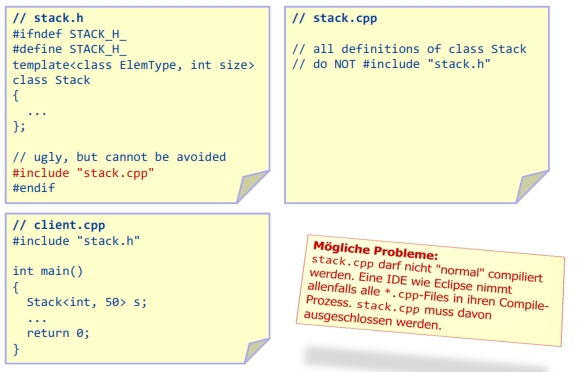
\includegraphics[width=0.9\textwidth]{pics/template_klasse_1.jpg}
		\end{minipage}
		\hspace*{0.5cm}
		\begin{minipage}[t]{9 cm}
			\subsubsection{M�glichkeit 2}
				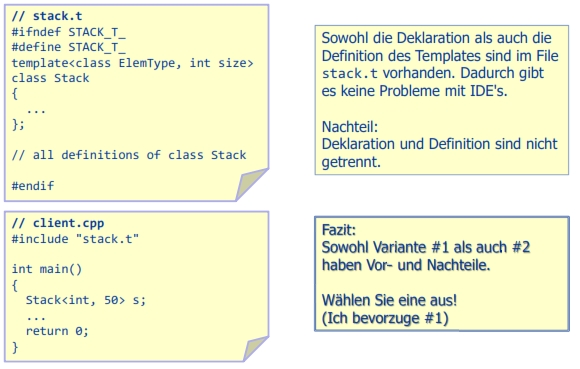
\includegraphics[width=0.9\textwidth]{pics/template_klasse_2.jpg}
		\end{minipage}